\documentclass{article} % For LaTeX2e
\usepackage{nips15submit_e,times}
\usepackage{hyperref,graphicx}
\usepackage{url}
\documentstyle[nips14submit_09,times,art10]{article} % For LaTeX 2.09


\title{A Multimodal Dialog System for Language Assessment: Current State and Future Directions}


\author{
David Suendermann-Oeft, Vikram Ramanarayanan, Zhou Yu, Yao Qian, Keelan
Evanini, Alexei Ivanov, Patrick Lange, Xinhao Wang, Klaus Zechner\thanks{ Use footnote for providing further information
about author (webpage, alternative address)---\emph{not} for acknowledging
funding agencies.} \\
Department of Computer Science\\
Cranberry-Lemon University\\
Pittsburgh, PA 15213 \\
\texttt{hippo@cs.cranberry-lemon.edu} \\
\And
Coauthor \\
Affiliation \\
Address \\
\texttt{email} \\
\AND
Coauthor \\
Affiliation \\
Address \\
\texttt{email} \\
\And
Coauthor \\
Affiliation \\
Address \\
\texttt{email} \\
\And
Coauthor \\
Affiliation \\
Address \\
\texttt{email} \\
(if needed)\\
}

% The \author macro works with any number of authors. There are two commands
% used to separate the names and addresses of multiple authors: \And and \AND.
%
% Using \And between authors leaves it to \LaTeX{} to determine where to break
% the lines. Using \AND forces a linebreak at that point. So, if \LaTeX{}
% puts 3 of 4 authors names on the first line, and the last on the second
% line, try using \AND instead of \And before the third author name.

\newcommand{\fix}{\marginpar{FIX}}
\newcommand{\new}{\marginpar{NEW}}

%\nipsfinalcopy % Uncomment for camera-ready version

\begin{document}


\maketitle

\begin{abstract}
 We present work in progress on a multimodal dialog system for English
language assessment using a modular cloud-based architecture adhering to
open industry standards.  Among the modules being developed for the
system, there are multiple which are heavily deploying machine learning
techniques, including speech recognition, spoken language proficiency
rating, speaker verification, and the scoring of behaviors in multimodal
data streams.
\end{abstract}

\section{Introduction}


Whether it is in a K-12 educational setting, a working environment, or
in the academic domains, learning the English language encompasses the
development of proficiency on the four traditional skills Reading,
Writing, Speaking, and Listening [Rosenfeld et al., 2001]. Multiple
traditional assessments of the speaking skills are based on test taker
responses to given stimuli [TOEFL, ?]. Typical stimulus material
includes text, speech, images, etc. used as basis for subsequent
questions directed to the test taker [?]. The spoken responses are then
recorded and assessed offline commonly by a human evaluator or, in
certain cases, by a machine algorithm [SpeechRater].

One of the apparent drawbacks of this offline assessment methodology is
that contents of test taker responses will be unknown to the test
run-time environment while the test is being conducted. That is, there
is no interactivity involved, limiting the type of skills and knowledge
present items can evaluate.  However, interactivity does play a
significant role in academic and professional work environments alike.
While scoring rubrics of most current tests do address speech delivery
(such as pronunciation, fluency), language (vocabulary, grammar), and
content, they do not cover interactive skills [?]. [Zhou's comment: This place we need literature to back up the claim, why we need to access interactive communication skills in terms of language ability assessing.]

This paper describes work towards a multimodal dialog system addressing
the aforementioned shortcomings by engaging in a dialog with a test
taker, without involving a human counterpart (the test administrator).
This bears the following advantages:
- reduced costs,
- no scheduling issues as the system is available 24/7,
- scalable solutions,
- reproducible decisions,
- detailed knowledge of and control over the scoring features used by
the system,
- no issues with fairness or bias based on the human-human interaction,
- use of input/output modalities other than just speech.

Section 2 briefly describes the architecture of the multimodal dialog
system which is based on the following five design principles:
- open-source (explain why), 
- cloud-based (explain why),
- distributed (explain why),
- industry-standard-compliant (explain why),
- modular (explain why).

While the current system adheres to traditional rule-based methods for
spoken language understanding and dialog management, multiple modules
have been prepared that make heavy use of data-driven methodologies
including
- a module for automated rating of spoken language (delivery,
vocabulary, grammar, and content), see Section 3,
- a module for verification of the speaker for enhancing test security,
see Section 4, and
- a module to evaluate test takers' behaviors using multimodal cues, see
Section 5.

Since several of these modules and their integration are still under
development, Section 6 will outline the next steps along the route
towards a full-blown multimodal assessment system, and how machine
learning can play a major role to accomplish this goal.
[Zhou's comment: how can all these sub-systems come together to contribute for a final concept. Does each system solve one particular missing link in language assessments]

\section{Multimodal Dialog System}
% [Vikram, Zhou, Alex]
% - brief introduction to MM Halef
% - brief description of example items
% - brief recap of data collection so far (including video)

\begin{figure*}[htb]
% \vspace{-20mm}
\centering
% \hspace{-9mm}
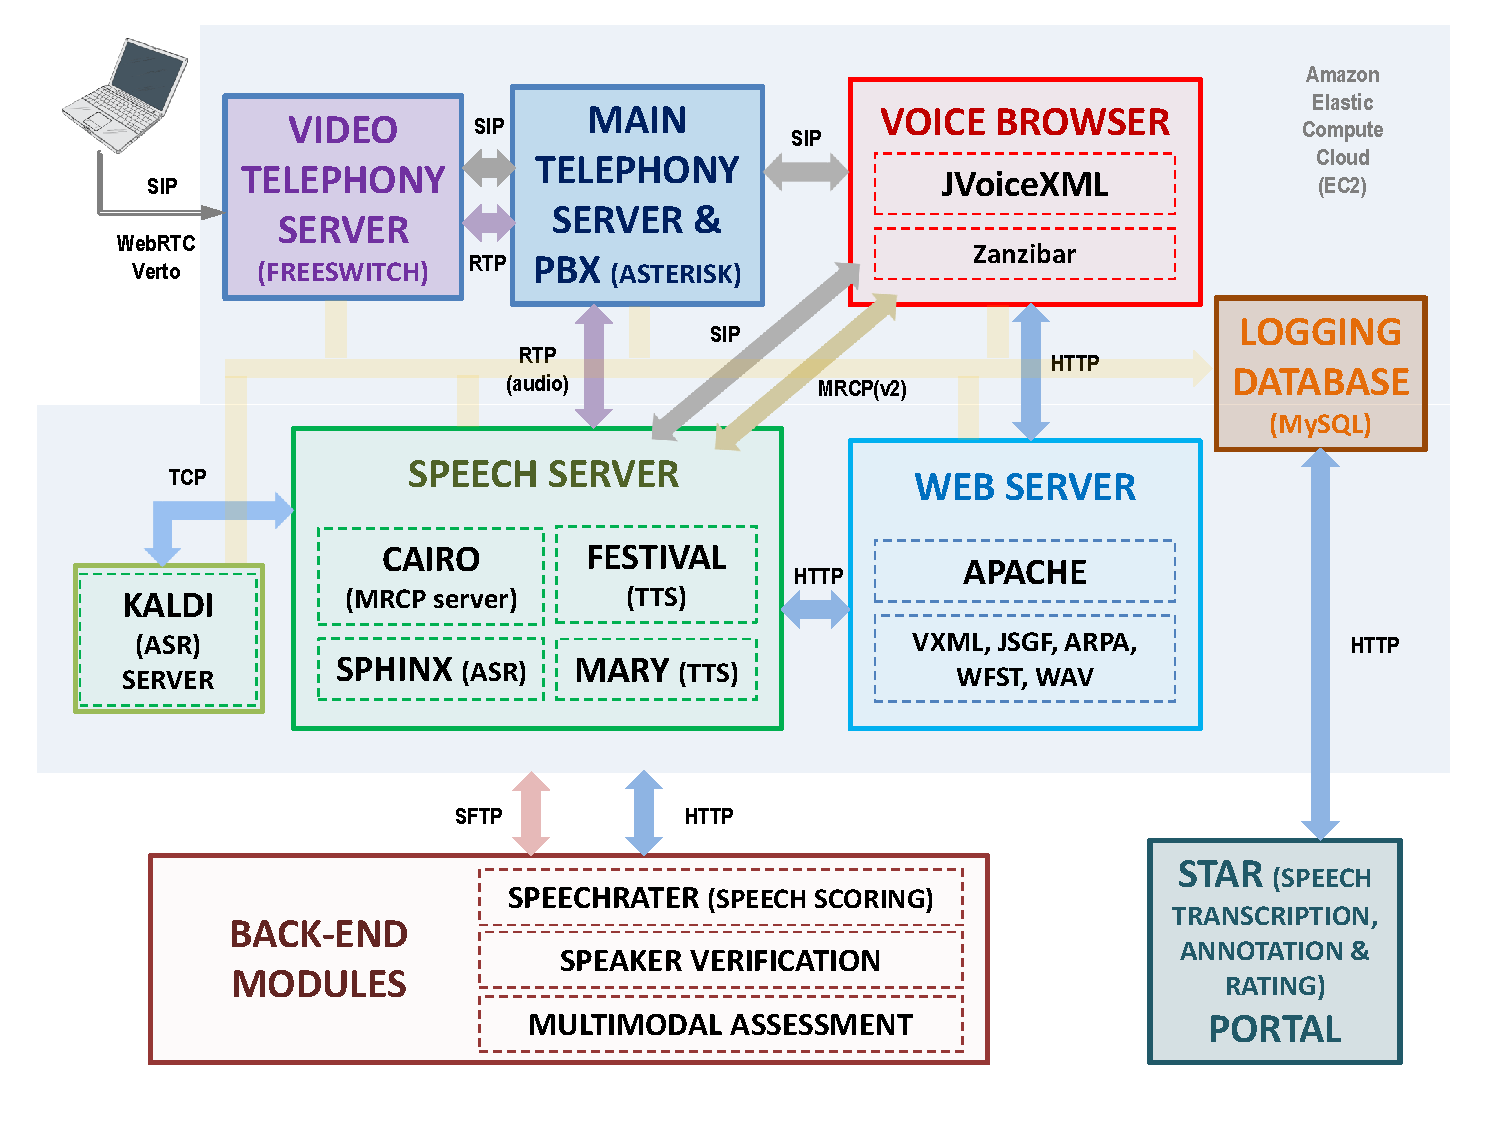
\includegraphics[scale=.50]{HALEF_v3_video_diffModules}
\vspace{-5mm}
\caption{System architecture of the HALEF multimodal dialog system depicting the various modular open-source components.}
\label{fig:HALEF}       
\vspace{-5mm}
\end{figure*}

\section{Speech Scoring}
% [Zhou, Xinhao]
For conversational assessment of spoken language, in particular formative assessment, it is desireable to use real-time automated speech scoring capabilities.
SpeechRater [Zechner et al.,2009] was the first system widely used for automatic non-native spontaneous speech scoring.  It consists of three main components, an automatic speech recognizer (ASR), a feature computation module, and the scoring model. The features used by SpeechRater are  manually designed to reflect aspects of pronunciation, fluency, intonation, rhythm, vocabulary use, and grammar while reflecting the very same rubrics human scorers evaluate.  This is to ensure fairness of automated assessments and prevents from test takers to capitalize on features correlated with the final score but with little construct relevance.

For our initial work on investigating the use of automated speech rating in spoken dialog systems, we relaxed the aforementioned constraint in favor of creating a real-time-able system.  To this end, we implemented a hybrid recurrent neural network framework which comes with minimal manual effort and cost, high scoring accuracy and speed [Yu et al.,2015].

In the proposed framework, we used generic time-sequence features extracted directly from the audio input instead of manually designed features, thus saving on human transcription effort and the expert knowledge for training and optimizing an ASR engine for the rater. The proposed framework also jointly optimizes the module for feature engineering and the module for scoring using a hybrid model of a bidirectional long short memory recurrent neural networks (BLSTM) and a multilayer perceptron (MLP). The BLSTM automatically learns the high level structure information from the basic prosodic features (e.g. pitch) and the mel frequency cepstral coefficients features (MFCCs). The MLP maps the features to a continuous score. The framework optimizes the BLSTM and MLP jointly using mini-batch stochastic gradient descent (SGD). The proposed framework achieved results comparable to the baseline SpeechRater model which requires human effort in designing the features and the computation overhead caused by the ASR module.

Another advantage of the proposed hybrid network structure is that it can use mini-batch SGD for optimization which is scalable with respect to the amount of training data. As a next step, we plan to increase the data size to up to 600,000 hours of non-native speech data available at ETS to explore the upper performance bound of the model.

%- brief description of SpeechRater
%- brief description of the work Zhou will present at ASRU, emphasizing
%on the great potential to use up to 600k hours of data available at ETS
%and the real-time ability of the decoder

\section{Speaker verification}
% [Yao, Alex]
% - brief explanation of why speaker verification is essential for
% enhancing test security
% - brief description of the work you submitted to ICASSP, emphasizing on
% the great potential to use up to 600k hours of data available at ETS for UBM training
In recent years, voice biometrics has been applied to detect fraudulent activity in language proficiency tests to enhance test security, thereby protecting the integrity of tests and ensuring valid test scores. Some of the possible scenarios for applying speaker recognition technology in language proficiency tests include the following: (a) comparing a test taker’s voice to a database of known impostors, (b) identifying potential impostors by speaker clustering across multiple test administrations, (c) verifying repeat test takers’ voices across test administrations, and (d) comparing a test taker’s voice with speech samples submitted at in a different context (e.g., at test registration or in a follow-up interview).

Applying voice biometrics to real-time spoken dialog systems used for spoken language assessment can provide additional benefits including (e) the ability to ask additional security questions in case the test taker's identity could not be verified, (f) adding an additional modality (such as video, as supported by the architecture prosented in this paper), or (g) requiring the test taker to provide additional documentation right after completing the test.

In conventional i-vector based speaker recognition systems [6],  speech utterances are first converted to a sequence of acoustic feature vectors, typically 20 dimensional mel-frequency cepstral coefficients (MFCC) and their dynamic counterparts; after that, speaker- and channel-independent super-vectors, which accumulate the zeroth, first and second order sufficient statistics, are computed by using the posterior probabilities of the classes from a pre-trained GMM-UBM;  next, the total variability matrix, T, is used to transform the super-vectors to the low dimensional i-vectors, which contain both speaker and channel variability; then linear discriminant analysis (LDA) is often used to do channel compensation; finally a score between the target and the test speaker (or impostor) is calculated by a scoring function such as probabilistic LDA (PLDA) for further compensation or by simply using the cosine distance. 

However, the conventional i-vector based speaker recognition systems may not be able to compare the speakers at the same phonetic content due to the unsupervised training used in GMM-UBM. Recently, speaker recognition systems with phonetically-aware DNNs have significantly outperformed standard i-vector based systems [7][8]. Phonetically-aware DNNs used for speaker recognition [9,10] mainly replace the GMM components with senones and utilize the corresponding posteriors from the senones to extract Baum-Welch statistics. Thus, the DNN models phonetic content (senones) in a supervised learning manner. It therefore allows the comparison among different speakers at the same phonetic content and then makes it easier to distinguish one speaker from the others compared to using a GMM-UBM.

There are many challenges in developing a unified system based on phonetically-aware DNNs for speaker recognition in the context of large-scale language assessment. For instance, test takers in a global assessment of English proficiency have a wide variety of L1 backgrounds, which makes it difficult to model all possible non-native accent patterns. In addition, the speech quality from different test centers can vary a lot due to various recording settings and environments. We investigate the DNN-based speaker recognition approach on a non-native spontaneous speech corpus for the purpose of test security. Noise-aware features and multi-task learning are investigated to improve the alignment of speech feature frames into the sub-phonemic “senone” space and to “distill” the L1 (native language) information of the test-takers into bottleneck features (BNFs), which we refer to as metadata sensitive BNFs. Experimental results show that the system with metadata sensitive BNFs can improve speaker recognition performance by an 11.4\% relative reduction in equal error rate (EER) compared to the baseline i-vector based system [9].


\section{Multimodal assessment}
% [Vikram]
% - brief explanation why multimodal data could be useful for assessment
% (e.g., which constructs in addition to the aforementioned traditional
% ones one could capitalize on)
% - brief recap of the ICMI results, emphasizing on the ones limited to
% speech and video (since these are the ones we are able to capture with
% MM Halef)

We recently presented [REF] a comparative analysis of three different feature sets -- time-aggregated Kinect features, time-series (or histograms of co-occurrence) Kinect features and SpeechRater features (this combines information from both across and within time-series) -- in predicting different human-rated scores of presentation proficiency. We found that certain scoring dimensions were better predicted by speech features, some on Kinect features, and others on combinations of all features. We further observed that these features allowed us to achieve prediction performance near human inter-rater agreement for a subset of these scores. Although there is much room for improvement along the lines of better, more interpretable and predictive features as well as machine learning algorithms and methods (indeed, we have only experimented with support vector regression here), these experiments provide us significant insight into understanding how to design better techniques for automated assessment and scoring of public speaking and presentation proficiency. 


\section{Conclusion and Outlook}
% [David, Keelan]


%% \subsection{Keywords for paper submission}
%% Your NIPS paper can be submitted with any of the following keywords (more than one keyword is possible for each paper):

%% \begin{verbatim}
%% Bioinformatics
%% Biological Vision
%% Brain Imaging and Brain Computer Interfacing
%% Clustering
%% Cognitive Science
%% Control and Reinforcement Learning
%% Dimensionality Reduction and Manifolds
%% Feature Selection
%% Gaussian Processes
%% Graphical Models
%% Hardware Technologies
%% Kernels
%% Learning Theory
%% Machine Vision
%% Margins and Boosting
%% Neural Networks
%% Neuroscience
%% Other Algorithms and Architectures
%% Other Applications
%% Semi-supervised Learning
%% Speech and Signal Processing
%% Text and Language Applications

%% \end{verbatim}


% \begin{table}[t]
% \caption{Sample table title}
% \label{sample-table}
% \begin{center}
% \begin{tabular}{ll}
% \multicolumn{1}{c}{\bf PART}  &\multicolumn{1}{c}{\bf DESCRIPTION}
% \\ \hline \\
% Dendrite         &Input terminal \\
% Axon             &Output terminal \\
% Soma             &Cell body (contains cell nucleus) \\
% \end{tabular}
% \end{center}
% \end{table}

% \begin{verbatim}
%   \usepackage[dvips]{graphicx} ... 
%   \includegraphics[width=0.8\linewidth]{myfile.eps} 
% \end{verbatim}
% or % Apr 2009 addition
% \begin{verbatim}
%   \usepackage[pdftex]{graphicx} ... 
%   \includegraphics[width=0.8\linewidth]{myfile.pdf} 
% \end{verbatim}


\subsubsection*{Acknowledgments}


\subsubsection*{References}


\small{
[1] Alexander, J.A. \& Mozer, M.C. (1995) Template-based algorithms
for connectionist rule extraction. In G. Tesauro, D. S. Touretzky
and T.K. Leen (eds.), {\it Advances in Neural Information Processing
Systems 7}, pp. 609-616. Cambridge, MA: MIT Press.

[2] Bower, J.M. \& Beeman, D. (1995) {\it The Book of GENESIS: Exploring
Realistic Neural Models with the GEneral NEural SImulation System.}
New York: TELOS/Springer-Verlag.

[3] Hasselmo, M.E., Schnell, E. \& Barkai, E. (1995) Dynamics of learning
and recall at excitatory recurrent synapses and cholinergic modulation
in rat hippocampal region CA3. {\it Journal of Neuroscience}
{\bf 15}(7):5249-5262.
}


[4]Yu, Z., Ramanarayanan, V., Suendermann-Oeft, D., Wang, X., Zechner, K., Chen, L., Tao, J. \& Qian, Y. (2015) Using Bidirectional LSTM Recurrent Neural Networks to Learn High-Level Abstractions of Sequential Features for Automated Scoring of Non-Native Spontaneous Speech, ASRU.

[5]Zechner, K., Higgins, D., Xi, X., \& Williamson, D. M. (2009). Automatic scoring of non-native spontaneous speech in tests of spoken English. Speech Communication, 51(10), 883-895.

[6]Dehak, N., Kenny, P., Dehak, R., Ouellet, P., \& Dumouchel, P. (2011). Front end factor analysis for speaker verification,”
IEEE Trans. Acoust., Speech, Signal Processing, vol. 19, no. 4, pp. 788–798.

[7]Lei, Y., Scheffer, N., Ferrer, L., \& McLaren, M. (2014). A novel scheme for speaker recognition using a phonetically-aware Deep Neural Networks, in Proc. of IEEE ICASSP 2014, pp. 1695–1699.

[8]Richardson, F., Reynolds,D. A., \& Dehak, N. (2015).  A unified Deep Neural Network for speaker and language recognition, in Proc. of Interspeech 2015, pp.1146-1150.

[9]Qian, Y., Tao, J., Suendermann-Oeft, D.,  Evanini, K., Ivanov, A. \& Ramanarayanan, V.  Metadata Sensitive Bottleneck Features for Speaker Recognition with Non-native Spontaneous Speech, submitted to ICASSP 2016.  
\end{document}
